\subsection{Электрические машины от Gimbal}
Прогресс в области механики, электроники и цифровых устройств, привел к созданию инновационных устройств. Это в свою очередь поспособствовало прогрессу, существенному повышению качества и возможностей ранее разработанных решений. Одним из примеров недавних разработок можно считать устройства группы gimbal[ссылка]. Устройство группы Gimbal изображенно на картинке 1.1 и представляет собой сложную систему взаимодействия электродвигателей, электроники и датчиков для обеспечения плавности и стабилизации камер. В большинстве случаев данные устройства используются людьми, поэтому уделяются особое внимание компактности и малому весу. 

\begin{figure}[H]
	\centering
	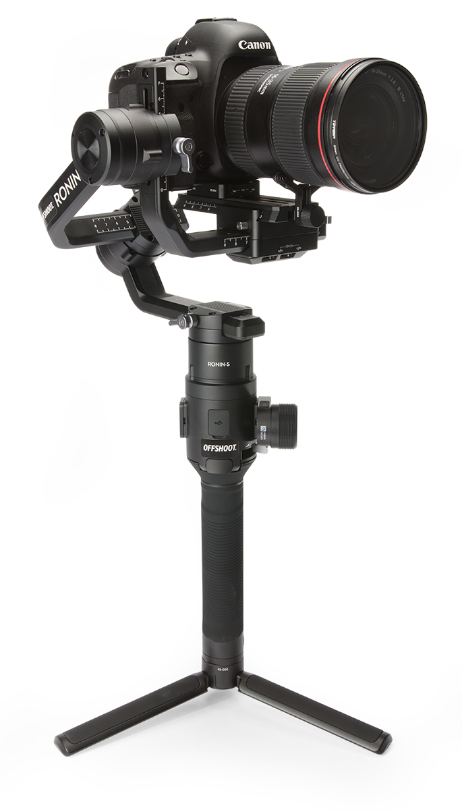
\includegraphics[width=0.3\textwidth]{Src/images/Gimbal.png}
	\caption{Устройство Gimbal}
\end{figure}

Главной особенностью является использование бесколлекторных электрических двигателей постоянного тока, известные также как BLDC (Brushless DC) моторы. BLDC моторы обладают высокой эффективностью и мощностью при небольшом весе. К примеру, стабилизатор камер «RONIN» от компании «DJI», можно считать популярными и доступным товаром на рынке. В его спецификации производитель заявляет максимальный вес до 7.25кг, при весе устройства (без груза)4.2 кг, то есть нагрузка превышает почти в более чем два собственный вес устройства 
\citep{ronin23}.

Данный пример не исключение, производители предлагают обширное количество моделей подобных устройств с различными характеристиками. Из-за высокого спроса на устройства данной категории, производители начали выпускать BLDC двигатели с оптимизированными параметрами электронных стабилизаторов. В интернете и литературе начали использовать термин Gimbal motors \citep{Lee2018}, то есть двигатели с конкретными характеристиками и под конкретные задачи. 

Существует интерес к разработкам различных типов BLDC моторов и возможности их использования при разработке робототехнических систем и устройств. Поэтому становиться актуальней задачей построение систем управления Gimbal для выполнения робототехнических операций.

\subsection{Особености мини роботов манипуляторов}

В настоящее время роботы манипуляторы являются главным элементом процесса автоматизации производств. Обуславливается это гибкостью, точностью, скоростью и способностью выполнять поставленные задачи. Роботы способны работать автономно круглосуточно, что способствует повышению количества производимых товаров. Роботы все больше используются для выполнения опасных, вредных и монотонных задач, облегчая условия труда для человека. Однако не во всех сферах роботы заменили ручной труд. Большинство работ связанных со сборкой деталей небольших размеров выполняются людьми. Для выполнения задач такого рода использование существующих универсальных индустриальных роботов является не эффективным и не рациональным решением, виду их большого размера и параметров несоотвествующих для работы с мелкими деталями и конструкциями.

Целесообразно использовать для задач подбора и размещения, сборки, дозирования, тестирования и контроля мелких деталей роботов меньших габаритов то есть мини роботов. Мини роботы манипуляторы существуют и разработки ведутся в данном направлении \citep{Li2022}, примером таких роботов могут считаться роботы моделей «MotoMini» от компании «Yaskawa» , «Meca500» (Рисунок 1.1) от компании «Mecademic»  и другие. Тема мини роботов не является новой, однако стоит отметить, количество информации, на данный момент, о роботах этого класса крайне не большое. В случае использования данных роботов в промышленном производстве в области работ с мелкими деталями, большинство задач требующих ручного труда человека, будут автоматизированы (робототизированны). 

\begin{figure}[H]
	\centering
	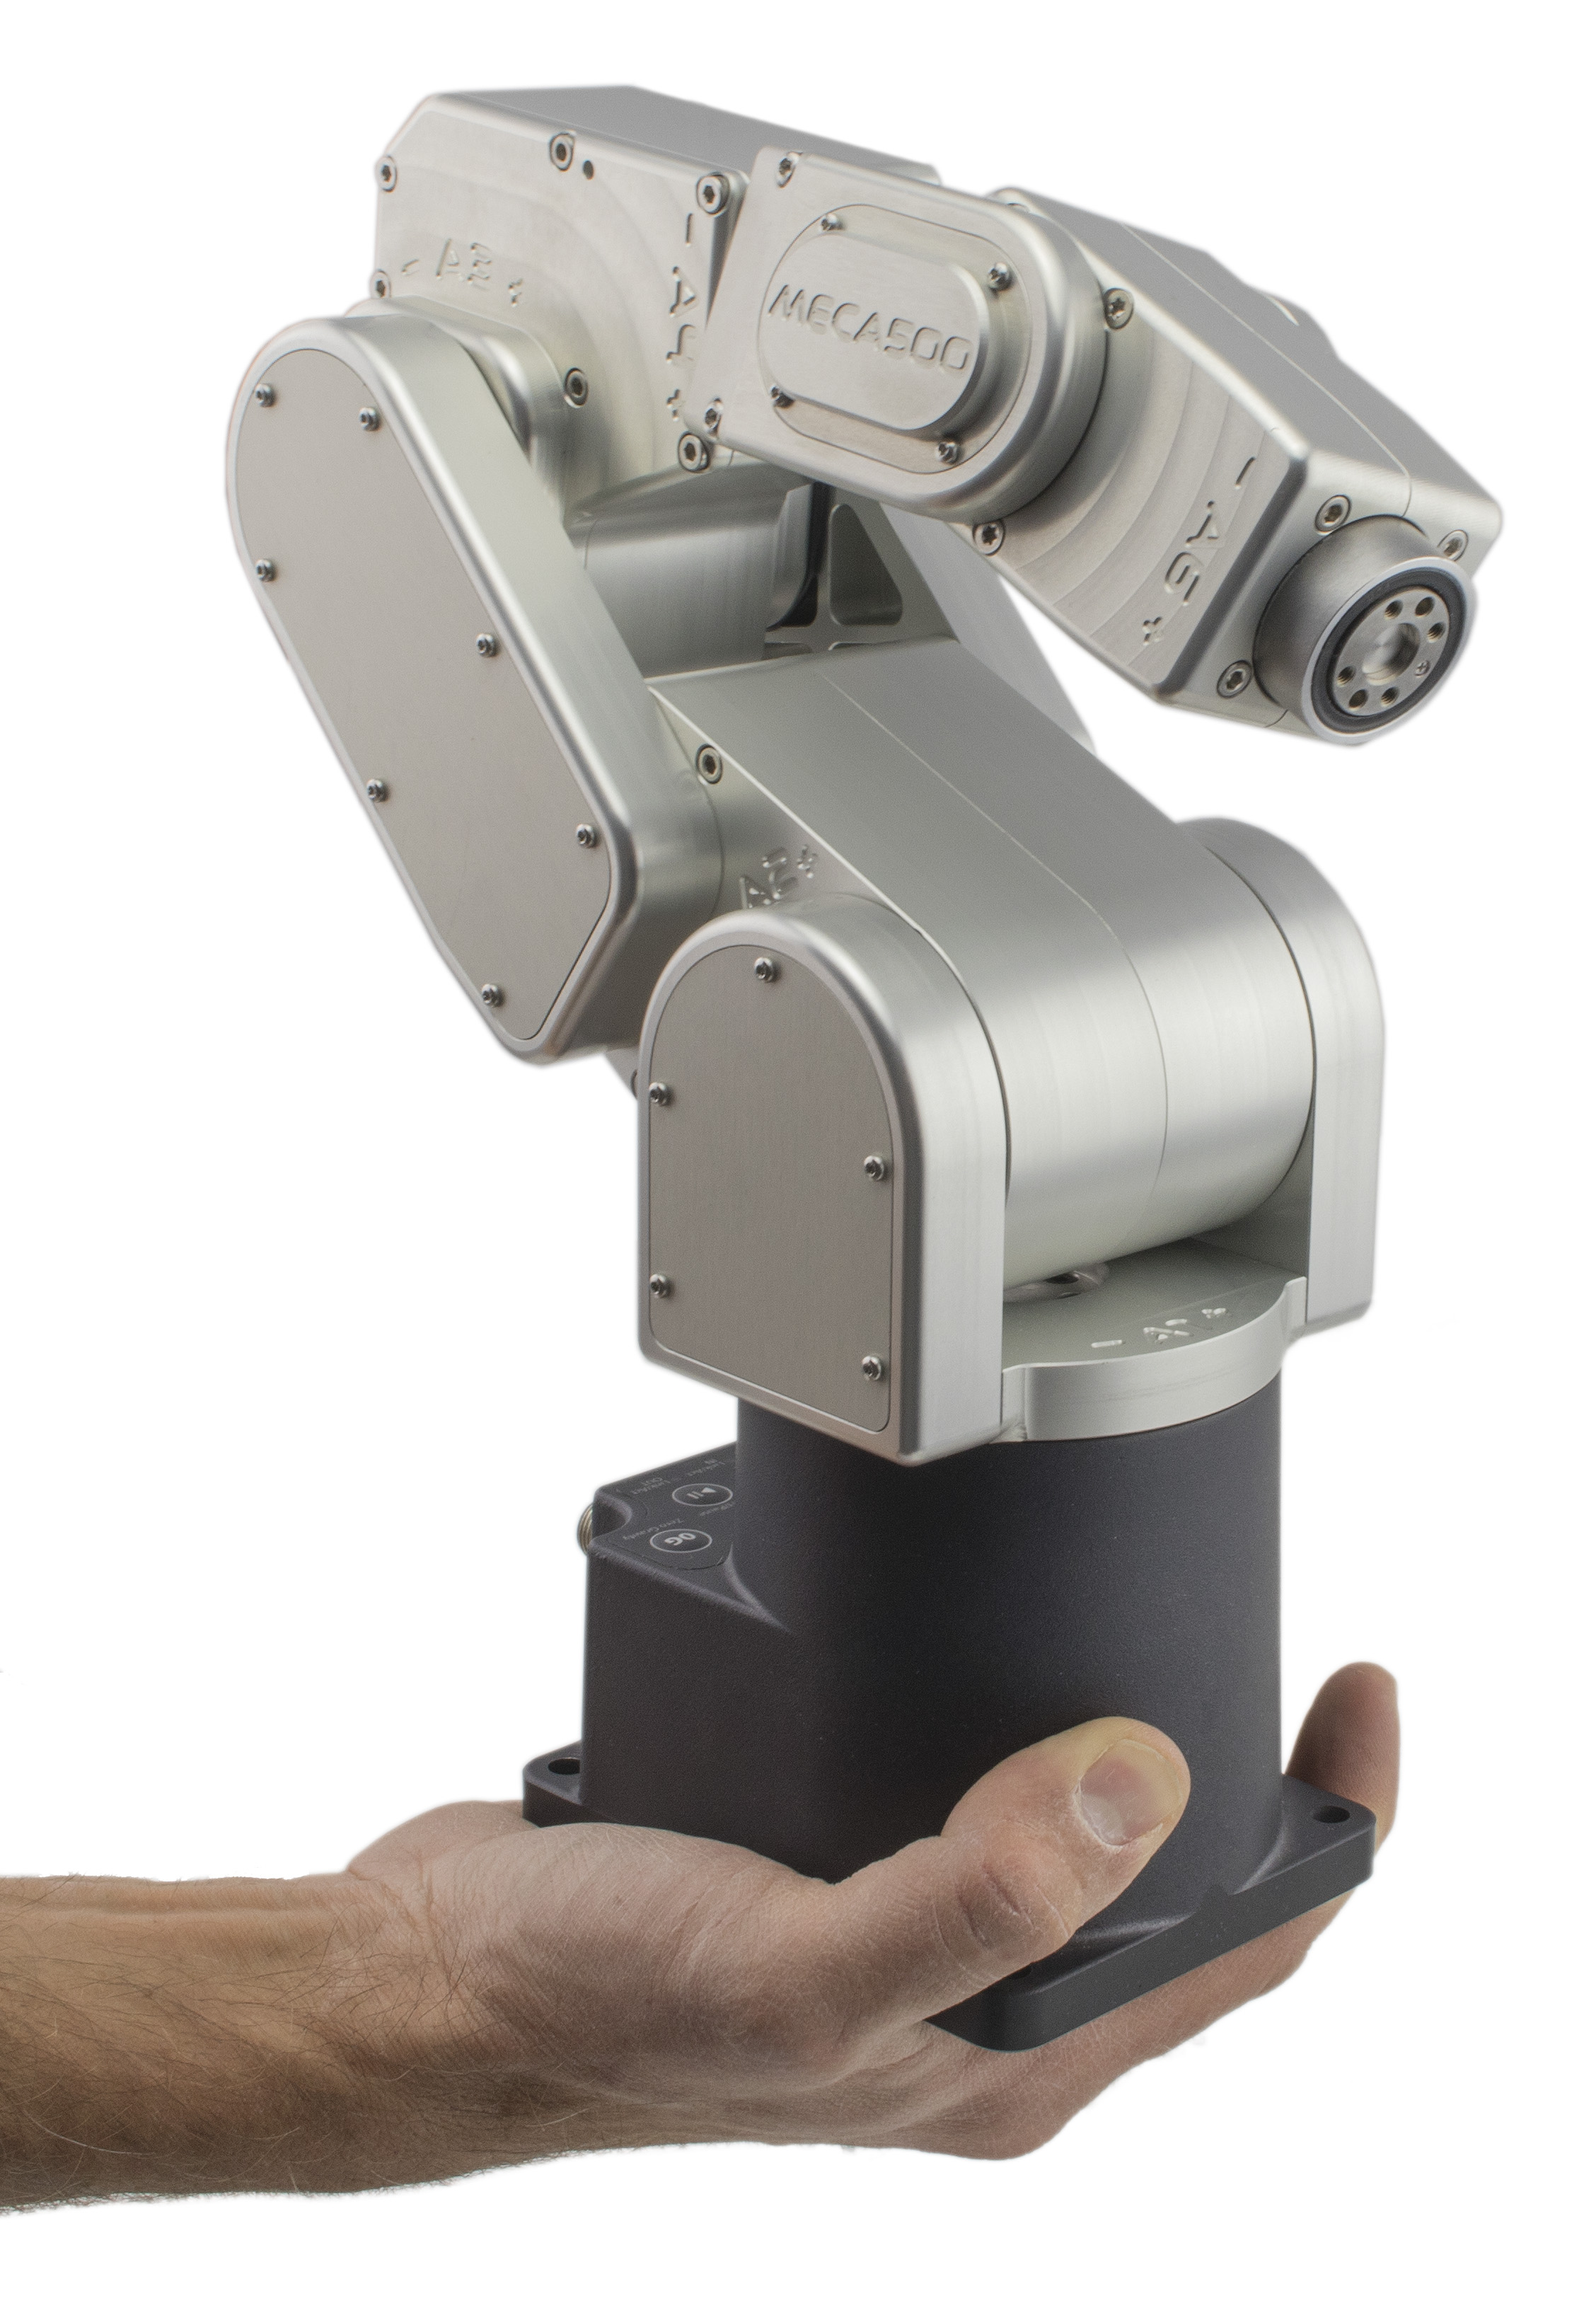
\includegraphics[width=0.3\textwidth]{Src/images/Meca500.jpg}
	\caption{Meca500 Robot Arm}
\end{figure}

На данный момент лидером в сфере промышленного производства является Китай, на промышленность которого приходится 32\% ВВП \citep[statistaChinaComposition] . Именно в Китае массовое производство является очень развитым. Главным фактором, обуславливающим это можно назвать то, что в КНР крайне дешевая рабочая сила (Рисунок 1.3). 

\begin{figure}[H]
	\centering
	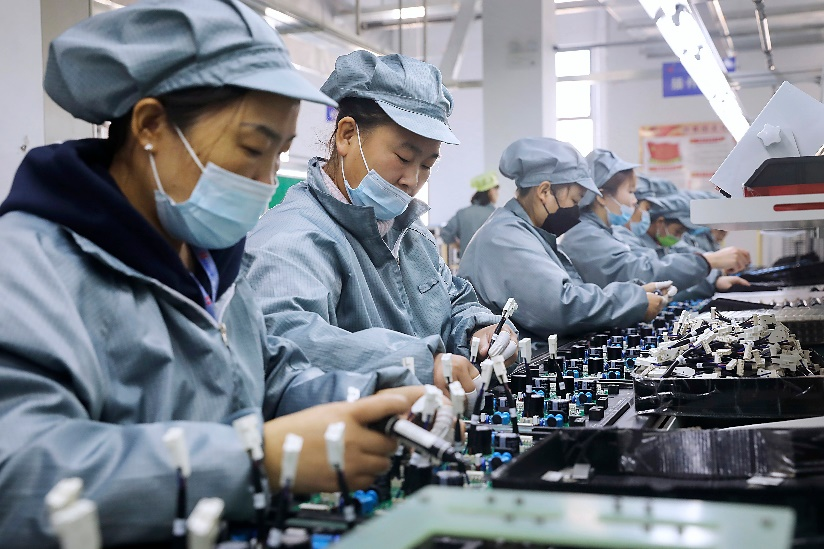
\includegraphics[width=0.7\textwidth]{Src/images/China.png}
	\caption{Процесс работы людей в Китае в сфере производства}
\end{figure}

Однако, за этим притягательным для многих, в том числе европейских, компаний фактором часто скрываются негуманные условия работы, детский труд и необеспечение безопасной рабочей среды. В свою очередь развитие мини роботов не только создаст почву для открытия промышленных производств в Евро Союзе, что в твою очередь уменьшит затраты на транспортировку и освободит от многих налогов, но и поможет предотвратить использование «грязной» рабочей силы.


Экономическая выгода для бизнеса от применения мини роботов большая, так как мини роботы способны заменить значимую часть человеческого ручного труда. Это в свою очередь создает благополучную почву для увеличения количества производимого товара, исключает большую часть возможных производственных ошибок, вызванных человеческим фактором. 

Замена рабочей силы может стать фактором для увеличения чистой прибыли компаний даже в Латвии, так как исключается необходимость в выплате обязательных взносов на национальное социальное страхование (MSSIC) размер которой составляет от 23,59 до 34,09 процентов ежемесячно.  Соответственно при уменьшении количества работников компания получит более высокий доход, ведь не будет необходимости платить суммарный налог MSSIC \citep{vid}.


Дальнейшее развитие мини роботов возможно только путем улучшении  их технических характеристик. При возможности использования компонентов малых размеров с требуемыми параметрами. Важным компонентом механизма мини робота манипулятора является электродвигатель. В поисках лучшего решения разрабатывают с различными вариантами двигателей. Исходя из тенденций последних исследований \citep{Sakama2022} рис 1.4 видно, что удельная мощность бесщеточных двигателей постоянного тока, с 1990-х годов, увеличилась более чем в десять раз за 20 лет, и теперь бесщеточные двигатели постоянного тока являются электродвигателями с самой высокой удельной мощностью. Удельная мощность данных двигателей увеличилась после появления постоянных магнитов с высокой максимальной энергией. В частности, появление неодимового магнита.

\begin{figure}[H]
	\centering
	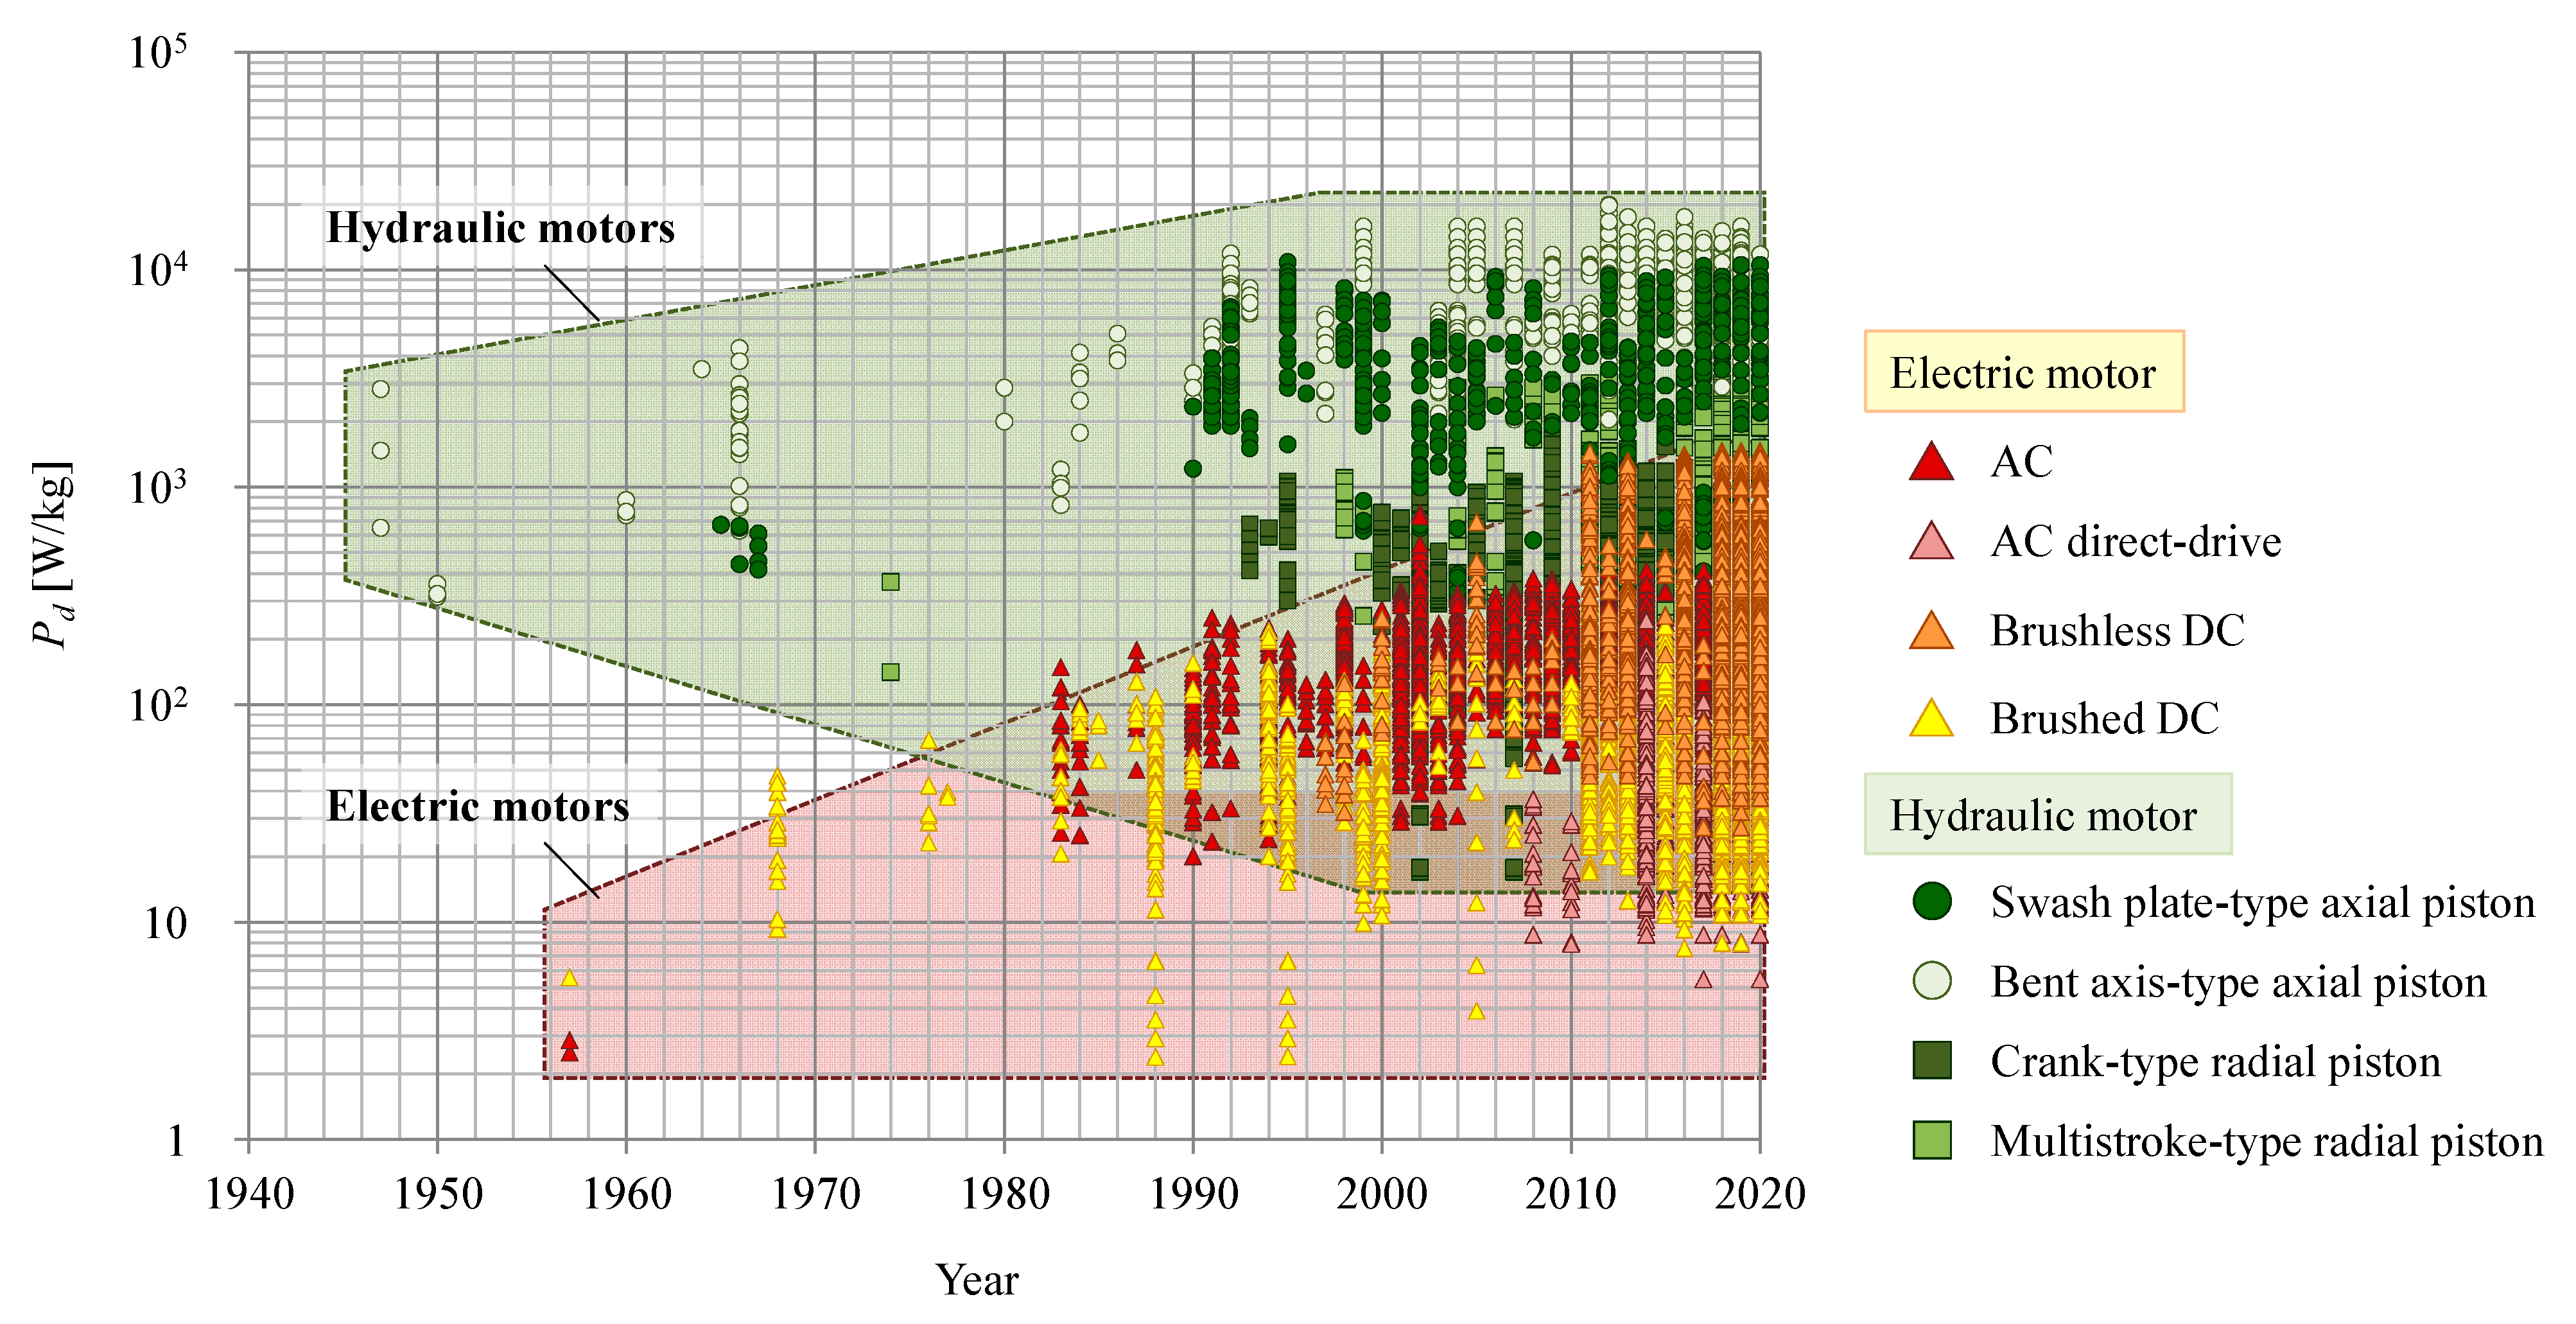
\includegraphics[width=\textwidth]{Src/images/magnets.png}
	\caption{Измерение удельной мощности в электрических двигателях во времени \citep{Sakama2022}}
\end{figure}

\subsection{ Общие требования к система управления робота манипулятора}

Любой робот-манипулятор состоит из различных систем: электронной, механической, вычислительной, сенсорной и других. Система управления робота должна организовывать работу между ними и обеспечить функционирование робота манипулятора по следующим требованиям:
\begin{itemize}
    \item Точное управление движением, плавное управление движениями робота с
        большой точностью, включая синхронизацию всех суставов и механизмов;

    \item Реализация заданных алгоритмов и задач, включает в себя задачи
        последовательности движений и операций действий робота;

    \item Обработка сенсорных данных, точно обрабатывать данные с датчиков для
        адаптации к изменениям окружающей среды;

    \item Взаимодействие с оператором, возможности для ручного управления и
        программирования;

    \item Интеграция с другими системами, робот являться не только одним
        элементом на производстве, использование совместно с системами конвейерных
        линий.
\end{itemize}

\subsection{Система управления Gimbal в роли системы управления роботом}

После тщательного изучения требований, которым должен соответствовать робот манипулятор. Возникает логичный вопрос: почему не использовать готовые наработки для стабилизации камер в робототехнике? Сравнительном анализ двух систем показывает методы и принципы управления в общем совпадают. Однако, более детальный анализ выявляет как потенциальные возможности, так и ограничения данного решения. Системы стабилизации камер, как и роботы-манипуляторы используют сложные алгоритмы для контроля положения и движения, но в случаях устройств Gimbal управление можно представить как величин питающего напряжения и частоты с использованием скалярных регуляторов. \citep{Altan2020} В тоже время области применения двух систем диаметрально отличаются друг от друга: в системах управлениях Gimbal не применяются датчики угла поворота оси двигателя, а информацию о значении текущего положении рассчитывается с использованием значений гироскопа и акселерометра. Значений этих датчиков достаточно для обеспечения стабилизации, но не достаточно для определения точного положения управляемого объекта в пространстве, причина тому наличие дрейфа получаемых данных \citep{1223234}.  Можно использовать алгоритмы фильтрования данных для уменьшения погрешностей управления, но это усложняет систему управления. Привлекательно является применение более простых и надёжных решения управления.

Если нет возможности использования систему управления от Gimbal по ряду причин, указанных выше, то тогда целесообразно разработать систему управления роботом на основе двигателей Gimbal Motors учитывая их достоинства (значительная мощность при маленьких габаритах) в системах стабилизации камер, а при учитывании актуальности использования мини роботов в целом. Актуальность разработки таких систем управления повышается в связи с тенденциями в необходимости разработок мини роботов и использование мини роботов в ближайшие годы.

Эта актуальность определила целью работы. Целью работы является разработка системы управления мини роботом манипулятором на основе Gimbal motors.